\documentclass{beamer}
%TODO:
%warum müssen wir supersingular curves benutzen?
%j-invariants
% wozu brauchen wir ramanujan graphs?

% Choose how your presentation looks.
%
% For more themes, color themes and font themes, see:
% http://deic.uab.es/~iblanes/beamer_gallery/index_by_theme.html
%
\mode<presentation>
{
  \usetheme{Madrid}      % or try Darmstadt, Madrid, Warsaw, AISEC ...
  \usecolortheme{default} % or try albatross, beaver, crane, ...
  \usefonttheme{default}  % or try serif, structurebold, ...
  \setbeamertemplate{navigation symbols}{}
  \setbeamertemplate{caption}[numbered]
} 

%\usepackage{fhgfont} funktioniert leider noch nicht
\usepackage[font=footnotesize]{caption} %for attributing pictures
\usepackage[english]{babel}
\usepackage[utf8x]{inputenc}
\usepackage{braket} % dirac notation
\usepackage{amsmath} % math symbols
\usepackage{amssymb} % other symbols
\graphicspath{ {img/} }
\usepackage{svg} %insert svg
\usepackage{svg-extract} %insert svg
\usepackage{graphicx} % insert pdfs
\newenvironment{rcases} % for right braces
{\left.\begin{aligned}}
	{\end{aligned}\right\rbrace}

\title[Shor's Algorithm]{SIKE - Supersingular Isogeny Key Encapsulation}
\author{Jonas von der Heyden}
\institute{FU Berlin}
\date{4.6.19}

\begin{document}
\newcommand{\source}[1]{\caption*{Source: {#1}} } %for attributing pictures
\begin{frame}
  \titlepage
\end{frame}

% Uncomment these lines for an automatically generated outline.
\begin{frame}{Outline}
  \tableofcontents
\end{frame}

\section{Introduction}

\begin{frame}{Introduction}

	\begin{itemize}
  		\item Goal of this presentation: Give a high-level overview of Shor's algorithm
	\end{itemize}

\end{frame}

\section{Mathematical primitive}

\subsection{Elliptic Curves}

\begin{frame}{Elliptic curves}
	Which figure is \textit{not} an elliptic curve?
	\begin{figure}
		\begin{minipage}{0.48\textwidth}
			\centering
			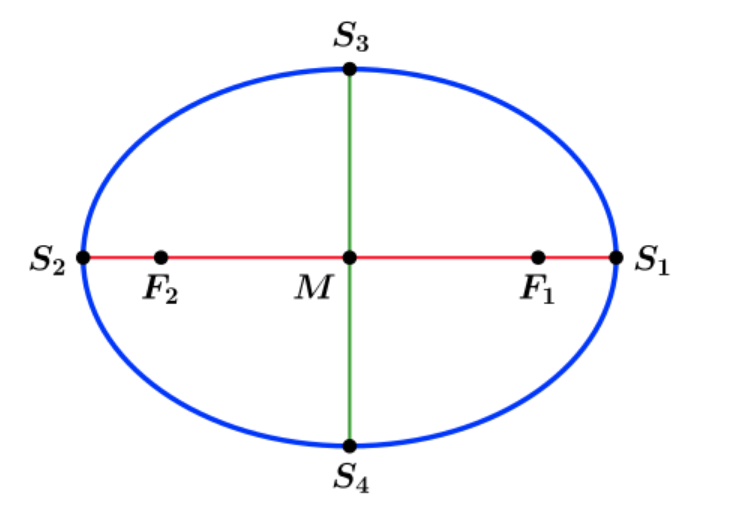
\includegraphics[width=.7\linewidth]{ellipse}
			\label{fig:ellipse}
		\end{minipage}\hfill
		\begin{minipage}{0.48\textwidth}
			\centering
			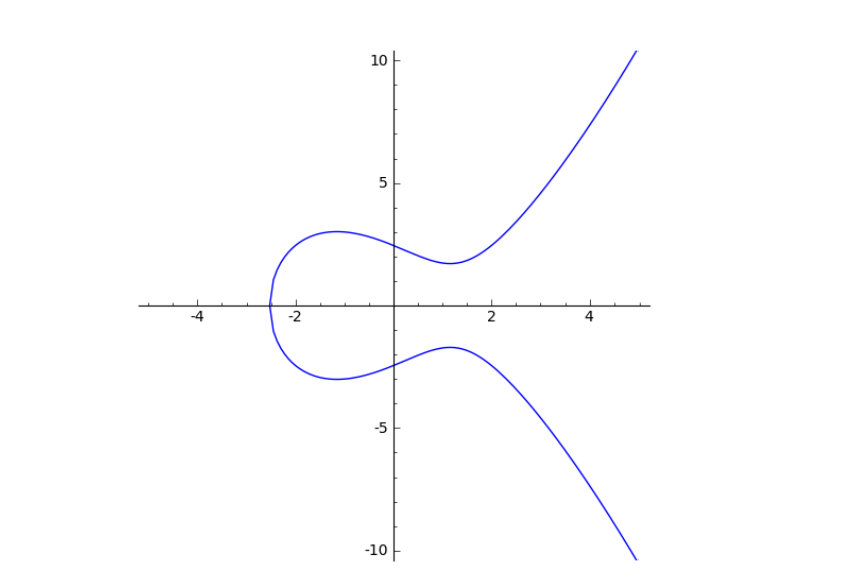
\includegraphics[width=.7\linewidth]{elliptic_curve}
			\label{fig:elliptic_curve}
		\end{minipage}
	\end{figure}
	\begin{figure}
	\begin{minipage}{0.48\textwidth}
		\centering
		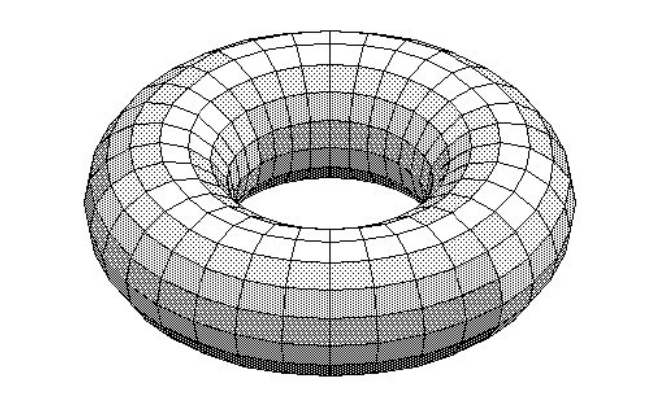
\includegraphics[width=.7\linewidth]{elliptic_curve_c}
		\label{fig:elliptic_curve_c}
	\end{minipage}\hfill
	\begin{minipage}{0.48\textwidth}
		\centering
		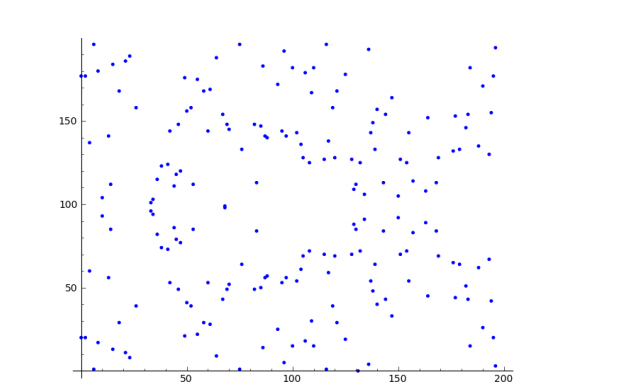
\includegraphics[width=.7\linewidth]{elliptic_curve_fp}
		\label{fig:elliptic_curve_fp]}
	\end{minipage}
\end{figure}


	% image of ellipse
\end{frame}

\begin{frame}{Elliptic curves}
	Which figure is \textit{not} an elliptic curve?
\begin{figure}
	\begin{minipage}{0.48\textwidth}
		\centering
		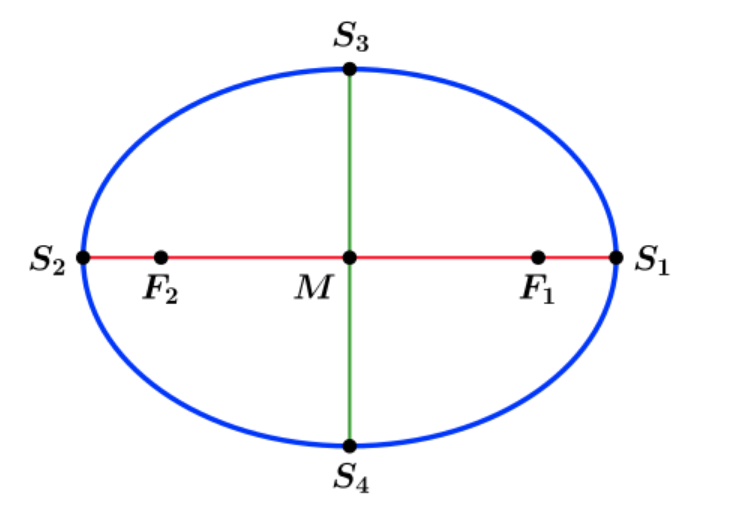
\includegraphics[width=.7\linewidth]{ellipse}
		\caption{Ellipse}\label{fig:ellipse}
	\end{minipage}\hfill
	\begin{minipage}{0.48\textwidth}
		\centering
		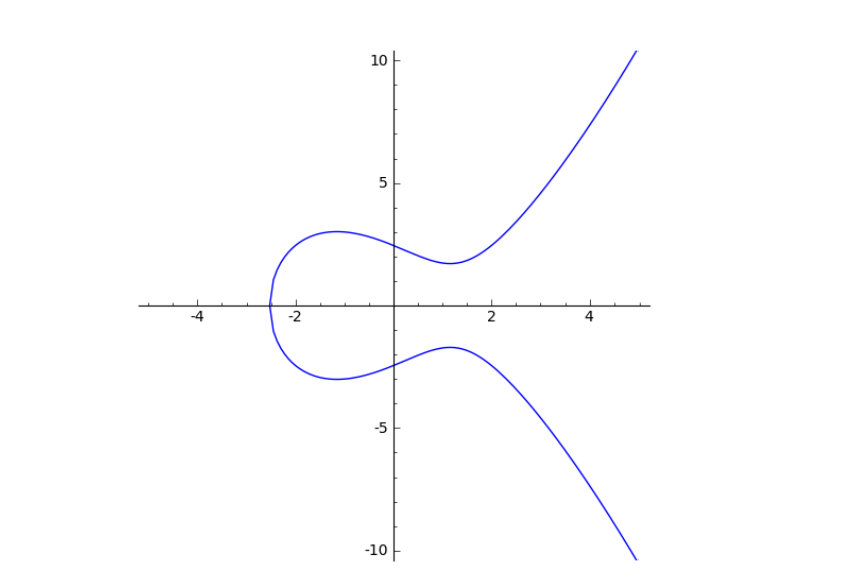
\includegraphics[width=.7\linewidth]{elliptic_curve}
		\caption{Elliptic Curve over $\mathbb{R}$}\label{fig:elliptic_curve}
	\end{minipage}
\end{figure}
\begin{figure}
	\begin{minipage}{0.48\textwidth}
		\centering
		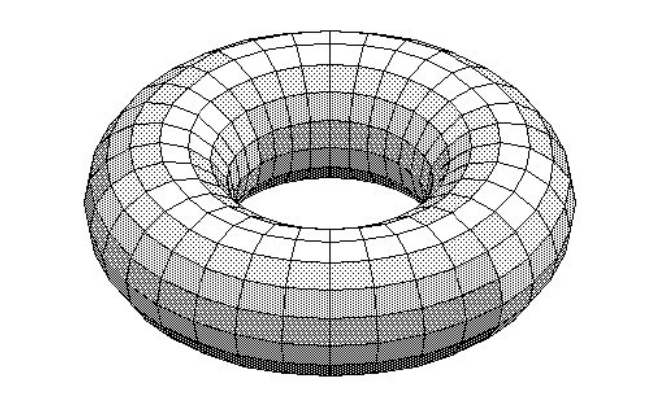
\includegraphics[width=.7\linewidth]{elliptic_curve_c}
		\caption{Elliptic Curve over $\mathbb{C}$}\label{fig:elliptic_curve_c}
	\end{minipage}\hfill
	\begin{minipage}{0.48\textwidth}
		\centering
		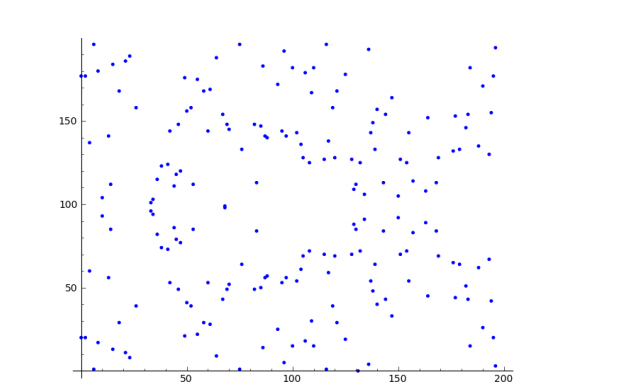
\includegraphics[width=.7\linewidth]{elliptic_curve_fp}
		\caption{Elliptic Curve over $\mathbb{F}_p$}\label{fig:elliptic_curve_fp]}
	\end{minipage}
\end{figure}

\end{frame}
\begin{frame}{Elliptic curves}
What is an elliptic curve?
\begin{itemize}
	\item Historically, elliptic curves were used to calculate the circumference of an ellipse
	\item An elliptic curve is the set of solutions to a \textit{Weierstrass equation} of the form $Y^2=X^3+AX+B$
\end{itemize}

\begin{figure}
	\centering
	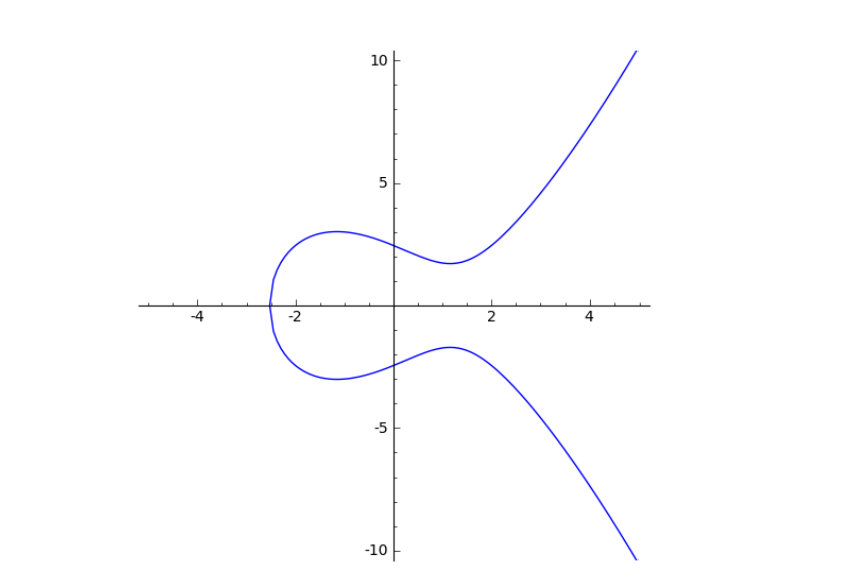
\includegraphics[width=.7\linewidth]{elliptic_curve}
	\label{fig:elliptic_curve}
\end{figure}
	
\end{frame}

\begin{frame}{Abelian Groups (G,+) over Elliptic Curves}
\begin{figure}
	\begin{minipage}{0.5\textwidth}
		\centering
		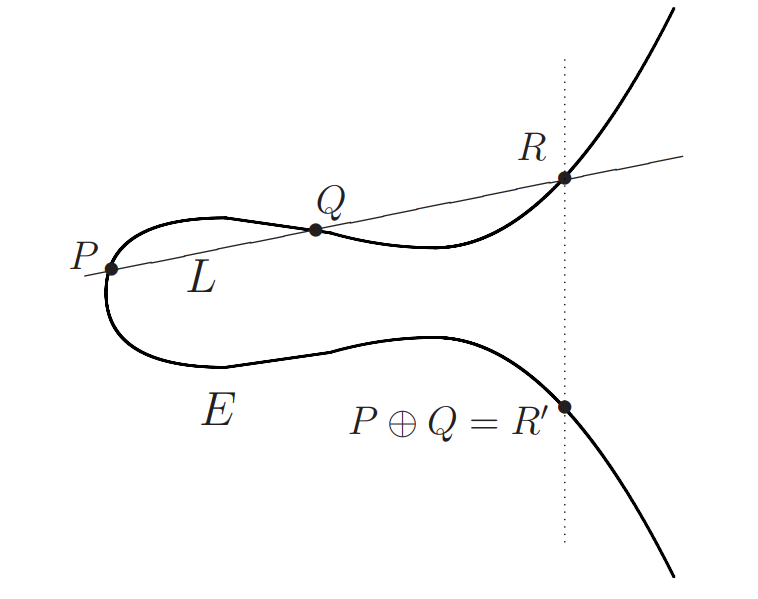
\includegraphics[width=1\linewidth]{P+Q}
		\caption{P+Q}\label{fig:p+q}
	\end{minipage}\hfill
	\begin{minipage}{0.48\textwidth}
		\centering
		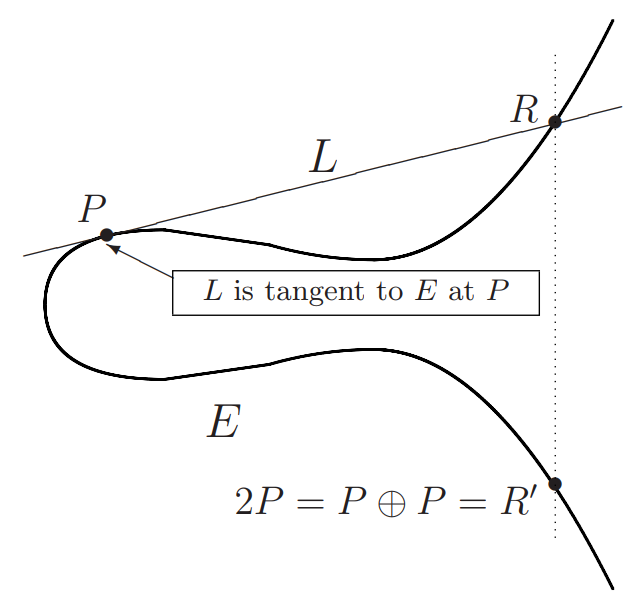
\includegraphics[width=1\linewidth]{P+P}
		\caption{P+P}\label{fig:p+p}
	\end{minipage}
\end{figure}

\end{frame}
\begin{frame}{Abelian Groups (G,+) over Elliptic Curves}
\begin{figure}

		\centering
		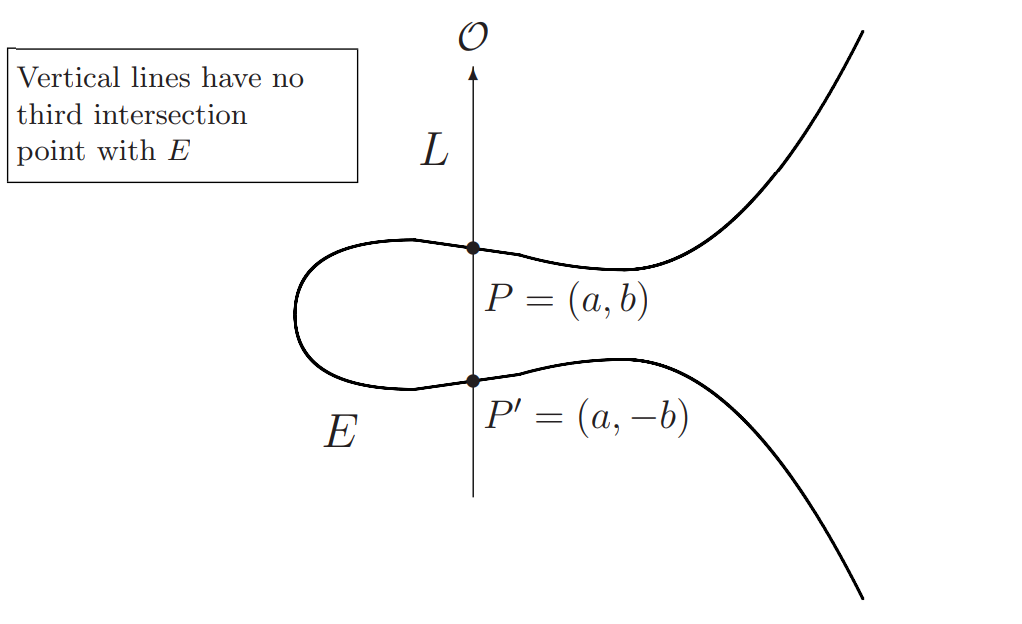
\includegraphics[width=1\linewidth]{P-P}
		\caption{P-P}\label{fig:p-p}


\end{figure}
\end{frame}
\begin{frame}{Abelian Groups (G,+) over Elliptic Curves}
	Let E be an elliptic curve. Then the addition law on E has the following properties:
	\begin{enumerate}
		\item $P + \mathcal{O} = \mathcal{O} + P$ (Identity)
		\item $P + (-P) = \mathcal{O}$ (Inverse)
		\item $(P + Q) + R = P + (Q + R) $ (Associative)
		\item $P + Q = Q + P$ (Commutative)
	\end{enumerate}

\end{frame}

\begin{frame}{Elliptic Curve addition algorithm}
	Let $E : Y^2 = X^3 + AX + B$ be an elliptic curve and let $P_1$ and $P_2$ be points on E.
	\begin{enumerate}
		\item If $P_1 = \mathcal{O}$, then $P_1 + P_2 = P_2$\pause
		\item Otherwise, if $P_2=\mathcal{O}$, then $P_1 + P_2 = P_1$\pause
		\item Otherwise, write $P_1 = (x_1,y_1)$ and $P_1 = (x_2,y_2)$\pause
		\item If $x_1 = x_2$ and $y_1=-y_2$, then $P_1+P_2=\mathcal{O}$\pause
		\item Otherwise, define \\
		\qquad \qquad \qquad$\lambda =
		\begin{cases}
			\frac{y_2-y_1}{x_2-x_1}\text{\quad if }P_1 \neq P_2\\\pause
			\\
			\frac{3x_1^2 +A}{2y_1}\text{\quad if }P_1=P_2 \pause
		\end{cases}$\\
		\vspace{5mm}
		and let $x_3=\lambda^2-x_1-x_2$  \hfill and $y_3=\lambda(x_1-x_3)-y_1$.\\
		\vfill
		Then $P_1+P_2=(x_3,y_3)$.
	\end{enumerate}
\end{frame}


\begin{frame}{Elliptic Curves over finite fields}
	\begin{itemize}
		\item An elliptic curve over $\mathbb{F}_p$ is an equation of the form $E:Y^2=X^3+AX+B$
		\item The set of points of E with coordinates in $\mathbb{F}_p$ is the set $E(\mathbb{F}_p)=\{(x,y):x,y\in \mathbb{F}_p$ satisfy $y^2=x^3+Ax+B \} \cup \{\mathcal{O}\}$
		\item Elliptic curve addition algorithm continues to work in $E(\mathbb{F}_p)$
		\item Addition law continues to satisfy properties of Abelian Groups
		\item If \#X is the cardinality of a set X, then \#$E(\mathbb{F}_q) = q+1-t$ for $|t|\leq 2\sqrt{q}$
		\item An elliptic curve $E(\mathbb{F}_q)$ is called \textit{supersingular} if $p \mid t$ where $q=p^a$
		\item It follows for all supersingular curves: $\#E(\mathbb{F}_q^n)\equiv 1 \bmod p$ for all $n\in \mathbb{N}$ and $p>3$
	\end{itemize}
	%TODO: (1)Beispiel!, (2) Konsequenz aus letztem Punkt
	
\end{frame}

\begin{frame}{ECDLP}
\end{frame}

\subsection{Points of finite order}

\begin{frame}{Points of finite order}
\begin{itemize}
	\item A point $P\in E$ satisfying $mP=\mathcal{O}$ is called a point of order m in the group E
	\item $E[m] = \{P\in E: mP = \mathcal{O}\}$ is also called the m-torsion group of E and includes all points of order $m$ in $E$
	\item $E[m] = \langle P \rangle $ is a subgroup of E since if $P,Q\in E[m]$ then also $P+Q$ and $-P$
\end{itemize}
 	
\end{frame}

\subsection{Isogenies}
\begin{frame}{Group homomorphisms}
Properties of group homomorphisms:
\begin{itemize}
	\item Given 2 groups (G,+), (H,$\oplus$) a group homomorphism is a function $\phi: G \to H$ such that $\phi(u + v) = \phi(u) \oplus \phi(v)$ 
	\item $\phi(e_G) = e_H$ where $e_G$ and $e_H$ are the identity elements of G and H
	\item The kernel of $\phi$ is the set of elements in $G$ which are mapped to the identity in $H$:
	$ker(\phi) \equiv \{u\in G:\phi(u)=e_H\}$
\end{itemize}
	 
	
	%Schaubild an Tafel
	\begin{block}{Example}
		$\phi: \mathbb{Z}\to\mathbb{Z}/3\mathbb{Z}$ is surjective and it's kernel consists of all elements in $\mathbb{Z}$ divisible by 3
		
		
	\end{block}
\end{frame}
\begin{frame}{Types of Homorphisms}
	\begin{itemize}
		\item Isomorphism: A group homomorphism that is bijective % Schaubild Graphisomorphie
		\item Endomorphism: A group homomorphism $\phi: G \to G$
		\item Isogeny: A group homomorphism $\phi : G \to H$ with a finite kernel
	\end{itemize}

\begin{block}{Isogeny Example}
	Multiplication map $[n]: E \to E$ defined by $[n]P = P + P + ...+ P$ ($n$ times):
	\begin{itemize}
		\item Maps 0 to itself and is surjective
		\item $ker[n] = E[n]$, therefore kernel is finite (if elliptic curve is defined over $\mathbb{F}_p$)
		\item Isogeny [n] can be calculated with elliptic curve addition algorithm %Beispiel an Tafel?
		
	\end{itemize}
%	Any 2 elliptic curves $E_1,E_2$ over $\mathbb{F}_q$ are isogenous iff $\#E_1(\mathbb{F}_q) = \#E_2(\mathbb{F}_q)$ ($E_1$ and $E_2$ have the same number of points). What about the kernel?
\end{block}

\end{frame}

\begin{frame}{Isogenies of elliptic curves}
Let $E_1,E_2$ be 2 elliptic curves over $\mathbb{F}_q$. Then an isogeny is a morphism $\phi: E_1 \to E_2$ s.t.:
\begin{itemize}
	\item $\phi(0_{E_1})= 0_{E_2}$
	\item $\#E_1(\mathbb{F}_q) = \#E_2(\mathbb{F}_q)$
	\item there exists a dual isogeny $\hat{\phi}: E_2 \to E_1$
	\item up to isomorphism it is uniquely defined by it's kernel $ker(\phi)$. Because a kernel is also a finite subgroup G of $E_1$ we can also say that $E_2$ is $E_1/G$
	\item equivalently it is also uniquely defined up to isomorphism by it's j-invariant $j(E)=1728\frac{4A^3}{4A^3+27B^2}$
	%how does j-invariant work?
\end{itemize}
\begin{block}{Example}
	% Example 3 aus Galbraith
\end{block}

\end{frame}
\begin{frame}{Endomorphism ring}


\end{frame}

\begin{frame}{Computing isogenies}
% galbraith p.6
\end{frame}

\section{Cryptosystem}

\subsection{SIKE protocol}

\begin{frame}{The SIKE protocol: Main idea}
Idea: Create Diffie-Hellman exchange over isogenies of elliptic curves. %DLDH an Tafel zeichnen
\begin{figure}
	\begin{minipage}{0.5\textwidth}
		\centering
		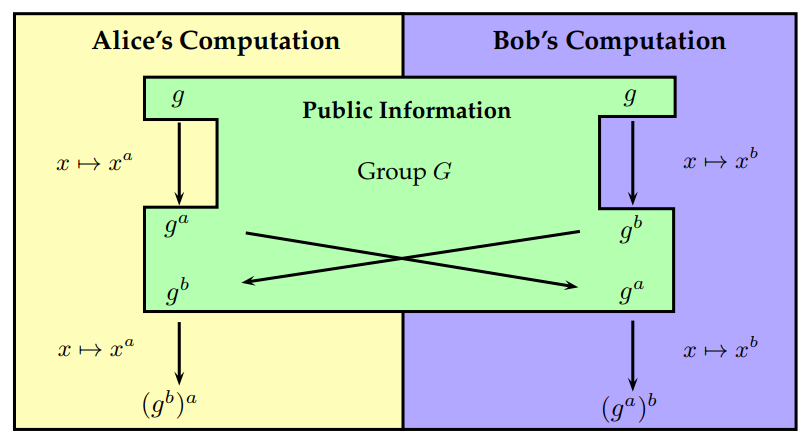
\includegraphics[width=1\linewidth]{DLDH}
		\caption{Discrete Logarithm Diffie-Hellman}\label{fig:dldh}
	\end{minipage}\hfill
	\begin{minipage}{0.48\textwidth}
		\centering
		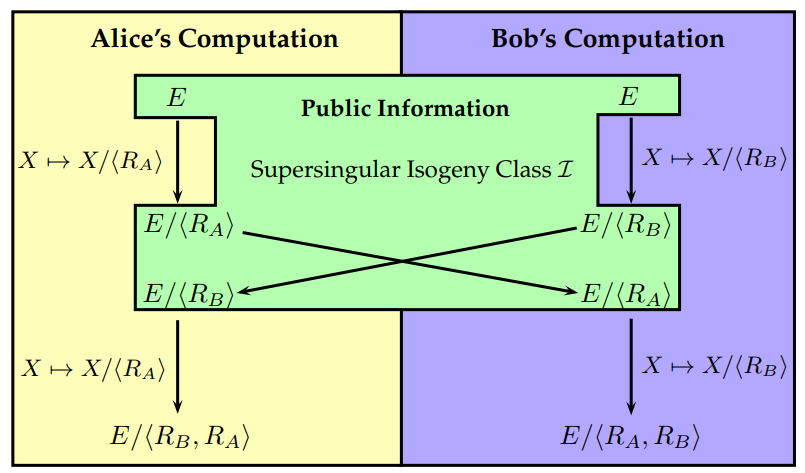
\includegraphics[width=1\linewidth]{SIDH}
		\caption{Supersingular Isogeny Diffie-Hellman}\label{fig:sidh}
	\end{minipage}
\end{figure}

\end{frame}
\begin{frame}{DH over isogenies of ordinary elliptic curves}

\end{frame}

\begin{frame}{The SIKE protocol: Walk-through}
\begin{enumerate}
	\item Generate Public Parameters:
	\begin{enumerate}
		\item Choose $2^{e_A},3^{e_B}$, search for a prime $p=2^{e_A}3^{e_B}f\pm 1$ and compute $q=p^2$
		\item Construct elliptic curve $E$ over $\mathbb{F}_q$ of cardinality $(2^{e_A}3^{e_B}f)^2$ %wie geht das?
		\item Find bases $P_A,Q_A$ and $P_B,Q_B$ that generate $E[2^{e_A}]$ and $E[3^{e_B}]$ respectively, s.t. $\langle P_A,Q_A\rangle$ = $E[2^{e_A}]$ and $\langle P_B,Q_B\rangle$ = $E[3^{e_B}]$ %wie schwierig ist das?
	\end{enumerate}
\end{enumerate}
\end{frame}
%TODO: visualization

\begin{frame}{Correctness}

\end{frame}

\subsection{Efficiency}

\begin{frame}{Composition chains of isogenies}
	% help to make computation of isogenies cheap: see Galbraith p.5
\end{frame}

\section{Areas of use}

\section{Security \& Complexity}
\subsection{SSDH assumption}


\section{Discussion}

\begin{frame}{Open questions}
\begin{itemize}
	\item Why do cryptosystem designers always choose extremly complicated problems that are not even NP-complete?
	\item Why not choose one of more than 1000 NP-complete problems? By definition they have a solution that is easy to verify but hard to compute.
\end{itemize}
\end{frame}

\begin{frame}{Questions?}
...
\end{frame}

\end{document}
